%\section{Motivation}
%\label{sec:motivation}
\section{Requirements for cellular in TVWS}
\label{sec:requirements}

%We start by explaining the requirements of a practical, long-range unlincensed cellular network and 
%examining whether existing technologies can fulfill these requirements. 
%We will focus on Wi-Fi and LTE radio technologies as most of today's high speed wireless networks are based on one of the two wireless standards.
%They incorporate most of the modern PHY and MAC layer design constructs which make them very efficient.
%Wi-Fi variant 802.11af is currently dominant among TVWS hardware platforms whereas LTE dominates the cellular market. 
%Furthermore, well developed designs and accompanying ecosystems make them most viable in business terms. 



\begin{table*}[htb!]
\centering
\begin{tabular}{  c || c | c | c | c || c | c | c  }
   & \multicolumn{4}{c ||}{{\bf PHY} (Section~\ref{sec:PHY})} & \multicolumn{3}{c}{{\bf MAC} (Section~\ref{sec:MAC})} \\ \hline
   %% & \multirow{2}{*}{Design} & Frequency & Coding & 
   %%   Hybrid & \multirow{2}{*}{Access} & \multirow{2}{*}{TX duration} & \multirow{2}{*}{Mode} \\ 
   %% & & chunks & rates & ARQ & & &  \\ \hline
   & {Design} & Freq. chunks & Coding rate & 
     Hybrid ARQ & Access & TX duration & Mode \\ \hline
  {\em 802.11af} & OFDM & 6-8 MHz & $\geq 0.5$ & no & CSMA & up to 4ms & uncoordinated \\ \hline  
  {\em LTE} & OFDMA & 180 kHz & $\geq 0.1$ & yes & Static & 1ms subframes & coordinated 
\end{tabular}
 \caption{Summary of differences between 802.11af and LTE}
  \label{tab:comp}
\vskip -6pt
\end{table*}



Our goal is to design an unlicenced cellular network that comprises the main advantages of the Wi-Fi and cellular. 
Such a network should thus be characterized by wide coverage and be amenable to unplanned deployments. 
We start by examining the requirements of a practical, long-range unlincensed cellular network.


\noindent{\bf Range.} One of the main requirements of an unlicensed cellular network, and its main differentiation against traditional Wi-Fi services is range. 
The TV white space spectrum promises cell range of 1km and above in unlicensed spectrum, as well as better indoor penetration~\cite{Rice_af}. 
We thus require a cell to have a coverage of at least 1km. 
We also require it to have high per-user throughput of at least 1 Mbps, as promised by universal broadband service in many countries~\cite{uni_broadband}.  

\noindent{\bf Database access compliance to unlicenced spectrum.}
The TV White space is currently available for commercial use in the US, Singapore and the UK, and other countries are working on the relevant regulations. 
However, rules for accessing TVWS spectrum bands are different than the ones regulating Wi-Fi bands. 
TVWS spectrum is available to unlicensed devices (secondary users) only in the absence of incumbents (TV and wireless microphones, also called primary users). 
No device is allowed to access the spectrum before checking spectrum availability in a database~\cite{Rice_af}. 
TVWS database compliance is thus an important aspect of the network design.

\noindent{\bf Unplanned deployment in unlicenced spectrum.}
% The other equally important aspect is support for uncoordinated, unplanned deployments. 
To achieve the ease of Wi-Fi deployments, we need support for unplanned, uncoordinated deployments. Since no one owns the spectrum, it is very likely 
that multiple networks will be deployed in the same area and will need to coexist without mandating central coordination, much like Wi-Fi networks coexist today. 

%{\bf BR: Do we want to discuss this or rely on the discussion in \cf section?}
Coexistence between disparate wireless technologies in the same spectrum is a hard challenge, and still not fully solved in practice for many technologies (e.g., Wi-Fi, Zigbee and Bluetooth). In fact, none of the current TVWS standards (802.11af, 802.22 and Weightless) attempts to solve inter-technology coexistence problem. 
In the same spirit, we will mandate decentralized interference management only among nodes using the same network technology, 
and assume that in the future, either one technology will prevail or that a database will make sure different technologies will occupy different, non-overlapping parts of spectrum. 

Furthermore, we require our unlicensed cellular design to work entirely in unlicensed spectrum and not require a licensed spectrum anchor, so that anyone, and not only cellular operators, can deploy it. This is in contrast to current LTE proposals for 5 GHz ISM bands \cite{lteuforum_lteu, jian2015coexistence, radisys-lte}. 

%% {\bf Power assymetry}. Finally, an unlicensed cellular network has to cope with power asymmetry. 
%% According to the current TVWS regulation in the US, UK, access points can transmit with powers of up to 4W whereas a client device is limited to a maximum of 100 mW. 
%% However, this asymetry goes beyond regulation, as client devices have far stricter limitations on radiation, heat disspation and battery consumption 
%% (typical cellular phone transmit power is limited to 200mW whereas cell transmit power can go up to tens of Watts). 





%% \subsection{WiFi and LTE preliminaries}
%% \label{sec:prelims}

%% Most of today's high speed wireless networks are based on one of the two wireless standards: LTE and Wi-Fi.  
%% These standards incorporate most of the modern PHY and MAC layer design constructs which make them very efficient.
%% Wi-Fi variant 802.11af is currently dominant among TVWS hardware platforms whereas LTE dominates the cellular market. Furthermore, well developed designs and accompanying ecosystems make them most viable in business terms. 

%% \noindent{\bf Wi-Fi} uses CSMA/CA to avoid interference from other transmitters. 
%% A station checks if the medium is idle for a period of time before each transmission.  
%% If a station detects a collision, implying contention in a network, it extends the idle period. 
%% This allows Wi-Fi to quickly detect and exploit idle channel, but at the same time introduces inefficiencies. 
%% 802.11af PHY is very similar to 802.11ac except that it uses 6MHz and 8MHz channels and works in TVWS frequencies.

%% \noindent{\bf LTE} consists of a set of base-stations and clients, called \emph{eNodeB}s and \emph{UE}s respectively in LTE jargon.  
%% clients share common resources, which are defined in frequency and time in terms of \emph{resource blocks} (RB), each 180 kHz wide and 1ms long. 
%% Both uplink and downlink resource blocks contain signaling, control and data elements spread out in frequency and time. 
%% The signaling elements (reference signals, synchronization signals) are inserted to allow clients to detect LTE transmissions and keep in sync. 
%% The access point is in charge of scheduling both uplink and downlink traffic. 
%% It assigns multiple RBs to various clients and the assignment is communicated over the control channel. 
%% This makes intra-cell LTE communication very efficient. 
%% However, lack of channel sensing limits coordination among neighboring cells.

%% %The data is transmitted in data elements. 


\section{Existing technologies \& unlicenced \\ cellular}
We focus on Wi-Fi and LTE radio technologies as most of today's high speed wireless networks, and in particular cellular and TVWS networks, are based on one of these two wireless standards.
They incorporate most of the modern PHY and MAC layer design constructs which make them very efficient.
%The Wi-Fi variant 802.11af~\cite{Rice_af} is currently dominant among TVWS hardware platforms whereas LTE dominates the cellular market. 
Furthermore, well developed designs and accompanying ecosystems make them most viable in business terms -- client devices with variants of LTE and \wf are available today for under \$50. 



\subsection{Physical layer and coverage}
\label{sec:PHY}


\begin{figure*}[t]
  \begin{minipage}{0.32\textwidth}
    \centering
    (a)
    \vskip -2pt
    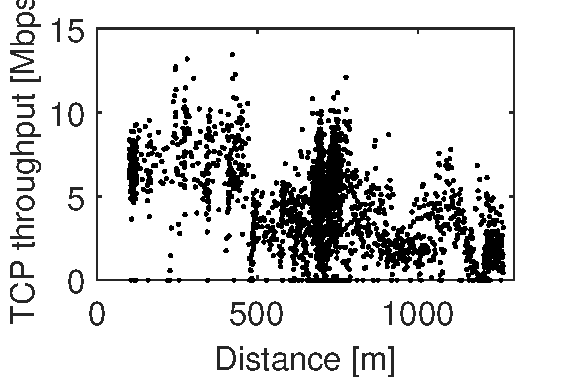
\includegraphics[width=\textwidth]{./figs/range.pdf}
  \end{minipage}
  \begin{minipage}{0.32\textwidth}
    \centering
    (b)
    \vskip -2pt
    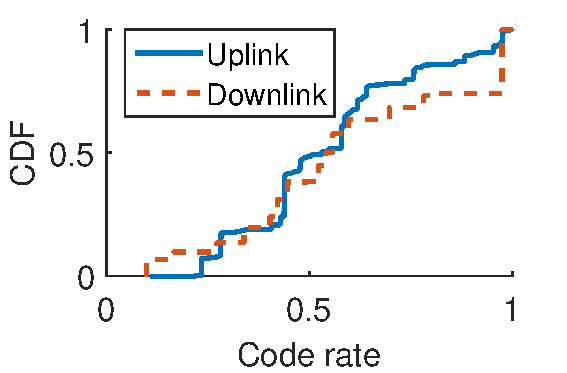
\includegraphics[width=\textwidth]{./figs/coding_rate.pdf}
  \end{minipage}
  \begin{minipage}{0.32\textwidth}
    \centering
    (c)
    \vskip -2pt
    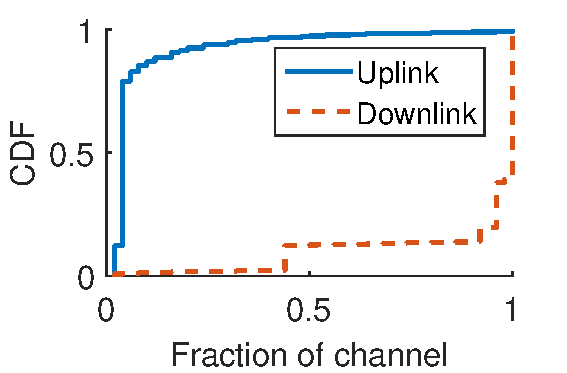
\includegraphics[width=\textwidth]{./figs/NRB.pdf}
  \end{minipage}
 \caption{Throughput as a function of distance (a), CDF of coding rate used (b) and fraction of channel used (c).}
  \label{fig:phy}
\vskip -6pt
\end{figure*}


LTE is based on OFDMA. Its clients share common resources, which are defined in frequency and time in terms of \emph{resource blocks} (RB), each 180 kHz wide and 1ms long. 
Both uplink and downlink resource blocks contain signaling, control and data elements spread out in frequency and time. 
The signaling elements (reference signals, synchronization signals) are inserted to allow clients to detect LTE transmissions and keep in sync. 
LTE PHY is designed for long range, so it contains features useful for low SNR links, such as low coding rates, hybrid ARQ and OFDMA modulation that allows 
the scheduler to use only a subset of resource blocks with the highest signal quality when sending to a specific client.

Most of the LTE hardware already works in a wide range of standardized 3GPP bands~\cite{36_101}. Some of these bands already coincide with TV white space frequencies in parts of the world (e.g., band 44 coincides with part of the TV white space spectrum in the UK). New 3GPP bands are likely to cover even more TV white space spectrum in future (e.g., future LTE bands to cover spectrum sold under US broadcast incentive auctions~\cite{fcc_600}). 
3GPP radio requirements~\cite{36_101, 36_104} adhere to ETSI TVWS spectral mask requirements~\cite{etsi_tvws}. 
Furthermore, the LTE PHY can use a single channel (in TDD mode) and allows for 5MHz, 10MHz, 15MHz and 20MHz bandwidths; it can thus adapt to several contiguous available TV channels (TV channels are 6MHz in the US and 8MHz in the EU). 

Wi-Fi PHY has originally been designed for short range. It uses OFDM, which means that only one client can be served at one time over the entire spectrum, regardless of signal quality on each subcarrier. Newest Wi-Fi standards (802.11ac) use high coding rates, the minimum being 1/2. 
The recent 802.11af~\cite{Rice_af} standard specifies amendments to 802.11 to allow WLAN to operate in the TVWS spectrum. The standard has opted to keep the main features of the 802.11 PHY in order to minimize the cost of modifications. 802.11af PHY uses 6MHz and 8MHz channels and works in TVWS frequencies. It has the same modulation and coding rates as 802.11ac. 

Table~\ref{tab:comp} summarizes the properties of the two technologies. To better understand the impact of these in practice for long-range, we perform an outdoor experiment. We are unable to find 802.11af hardware that operates in the frequencies that we have access to. Instead, we perform an experiment using LTE hardware and monitor the impact of key properties from Table~\ref{tab:comp}, such as OFDMA, coding rate and Hybrid ARQ, on coverage. We deployed an LTE small cell on the top of our building. We moved a client throughout the coverage area and recorded its location, the downlink TCP rate achieved using iperf and various LTE performance metrics (please see Section~\ref{sec:implementation} for a detailed description of this experiment). 

Figure~\ref{fig:phy} presents the results of the experiment. 
We observe that with 36dBm EIRP (29dBm transmit power and 6dBi directional antenna) at the AP and 20dBm transmit power at the client (maximum according to TVWS specs), LTE can reach 1.3km in the urban environment.
We measured and achieve 1Mbps TCP rates at more than 85\% of measured locations (in Figure~\ref{fig:phy}(a)). 
In order to achieve these ranges LTE frequently used very low coding rates (Figure~\ref{fig:phy}(b)). 
In fact, the median coding rate was 1/2, which corresponds to the lowest coding rate offered by 802.11af~\cite{Rice_af}. 
Further, LTE leverages its OFDMA capabilities and schedules  
uplink transmission consisting solely of TCP ACK packages which are small in size
in a single resource block. This is shown in Figure~\ref{fig:phy}(c), where we plot the CDF of the fraction of the channel used by transmissions.
LTE chooses the resource block with the highest signal strength and improves the quality of transmission -- this also explains why the LTE uplink and downlink used similar coding rates. 
In similar scenarios, WiFi would reduce the signal quality and consequently the range of the network, 
since it does not implement OFDMA and it would have to send uplink packets across the entire bandwidth. 
Finally, we observe that LTE leverages hybrid ARQ to improve communication quality, and in particular for longer links - we see that 25\% of packets sent from distances larger than 500m use hybrid ARQ. 

%Wi-Fi does not implement OFDMA and it will have to send uplink packets across the entire bandwidth, which will reduce the signal quality and consequently the range of the network. 

%In order to compare the performance of the two PHYs, , and evaluated its performance outdoors. 
%The results are depicted in Figure~\ref{fig:phy}. We were unable to get an 802.11af hardware at the time. Instead we look at the results of our experiments and compare with the main design point of 802.11af (see Table~\ref{tab:comp} for head-to-head comparison). %

%Secondly,, 

%Thirdly,. Uplink transmission consisted solely of TCP ack packages which are small in size, and LTE was able to leverage its OFDMA capabilities and schedule it in a single resource block. Consequently, it is also able to choose the resource block with the highest signal strength and improve the quality of transmission (which also explains why LTE uplink and downlink used similar coding rates). Wi-Fi does not implement OFDMA and it will have to send uplink packets across the entire bandwidth, which will reduce the signal quality and consequently the range of the network. 
%Finally, we observe that LTE leverages hybrid ARQ to improve communication quality, and in particular for longer links - we see that 25\% of packets sent from distances larger than 500m use hybrid ARQ. 

Overall, we see that the unique features of the LTE physical layer (as shown in Table~\ref{tab:comp}), namely, 
low coding rates, OFDMA medium access, and hybrid ARQ play a significant role in the LTE link quality and its ability to provide coverage of 1km and beyond. 



\subsection{Medium access and interference}
\label{sec:MAC}


%% \begin{figure}[t]
%%   \centering
%%     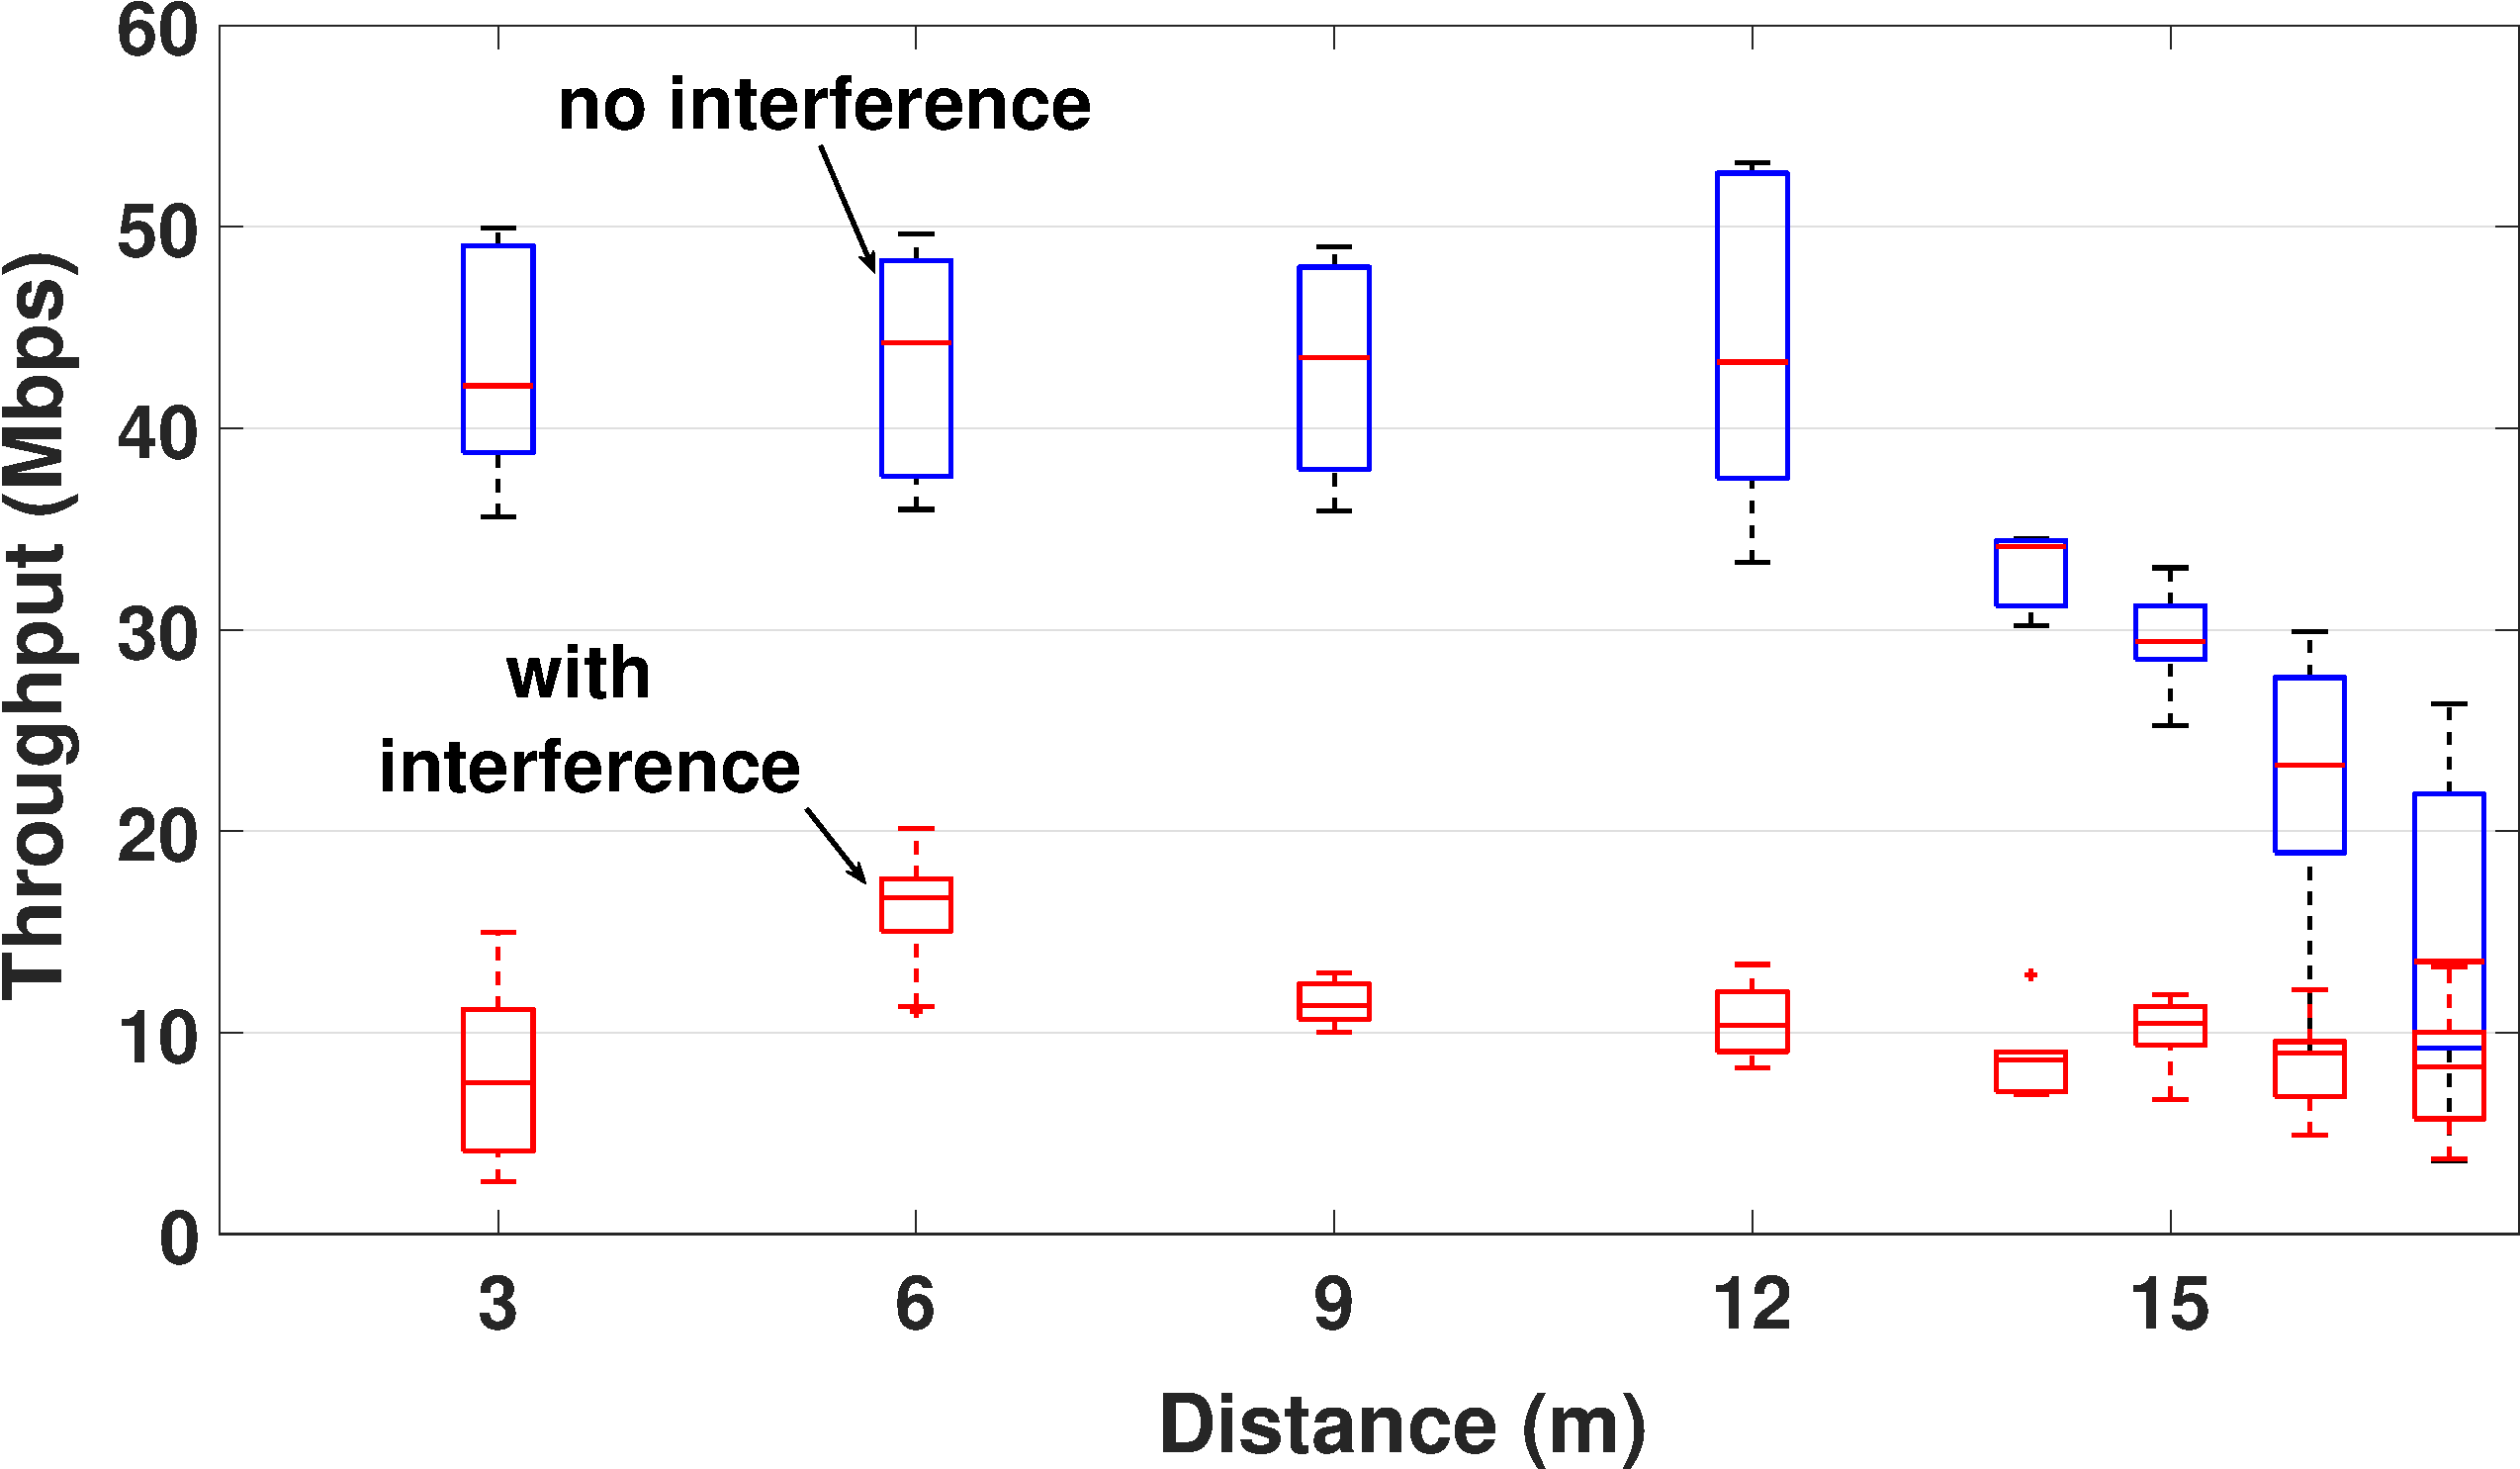
\includegraphics[width=0.5\textwidth, height=0.5\columnwidth]{./figs/interf_data-crop.pdf}
%%     \vspace{-0.3in}
%%   \caption{Throughput of a client with and without interference from an interfering access point. 
%%     The \emph{x-axis} refers to the distance from the serving access point.}
%%   \label{fig:interf}
%% \end{figure}


In LTE, an access point is in charge of scheduling both uplink and downlink traffic. 
It assigns multiple resource blocks to various clients and the assignment is communicated over the control channel. 
This makes intra-cell LTE communication very efficient. 
LTE assumes no unexpected interference from other networks; 
LTE deployments are well-planned and placement and configuration of access points is such that interference is managed in a coordinated fashion, 
either from a central network controller or through explicit coordination between neighbouring access points
(e.g., through X2 protocols~\cite{36_423}).

In an unlicensed band, these assumptions no longer holds true, as we can witness in numerous unplanned Wi-Fi deployments whose owners make no effort to optimize them. 
Regulators have also stirred clear from using a TVWS spectrum database to manage interference between unlicensed, secondary users. 
LTE offers no mechanisms to mitigate interference in uncoordinated deployments, where interference can significantly reduce performance. 
We illustrate this in detail in an experiment described in Figure~\ref{fig:interf_control} in Section~\ref{sec:interfeval},
where we show that a strong interferer (with SINR $\leq 10$ dB) can degrade LTE throughput by up to $2\times$, and also cause frequent disconnections. 
Thus, in order to make unplanned LTE deployment efficient, one needs to manage interference. 




%% \begin{figure}[t]
%%   \centering
%%     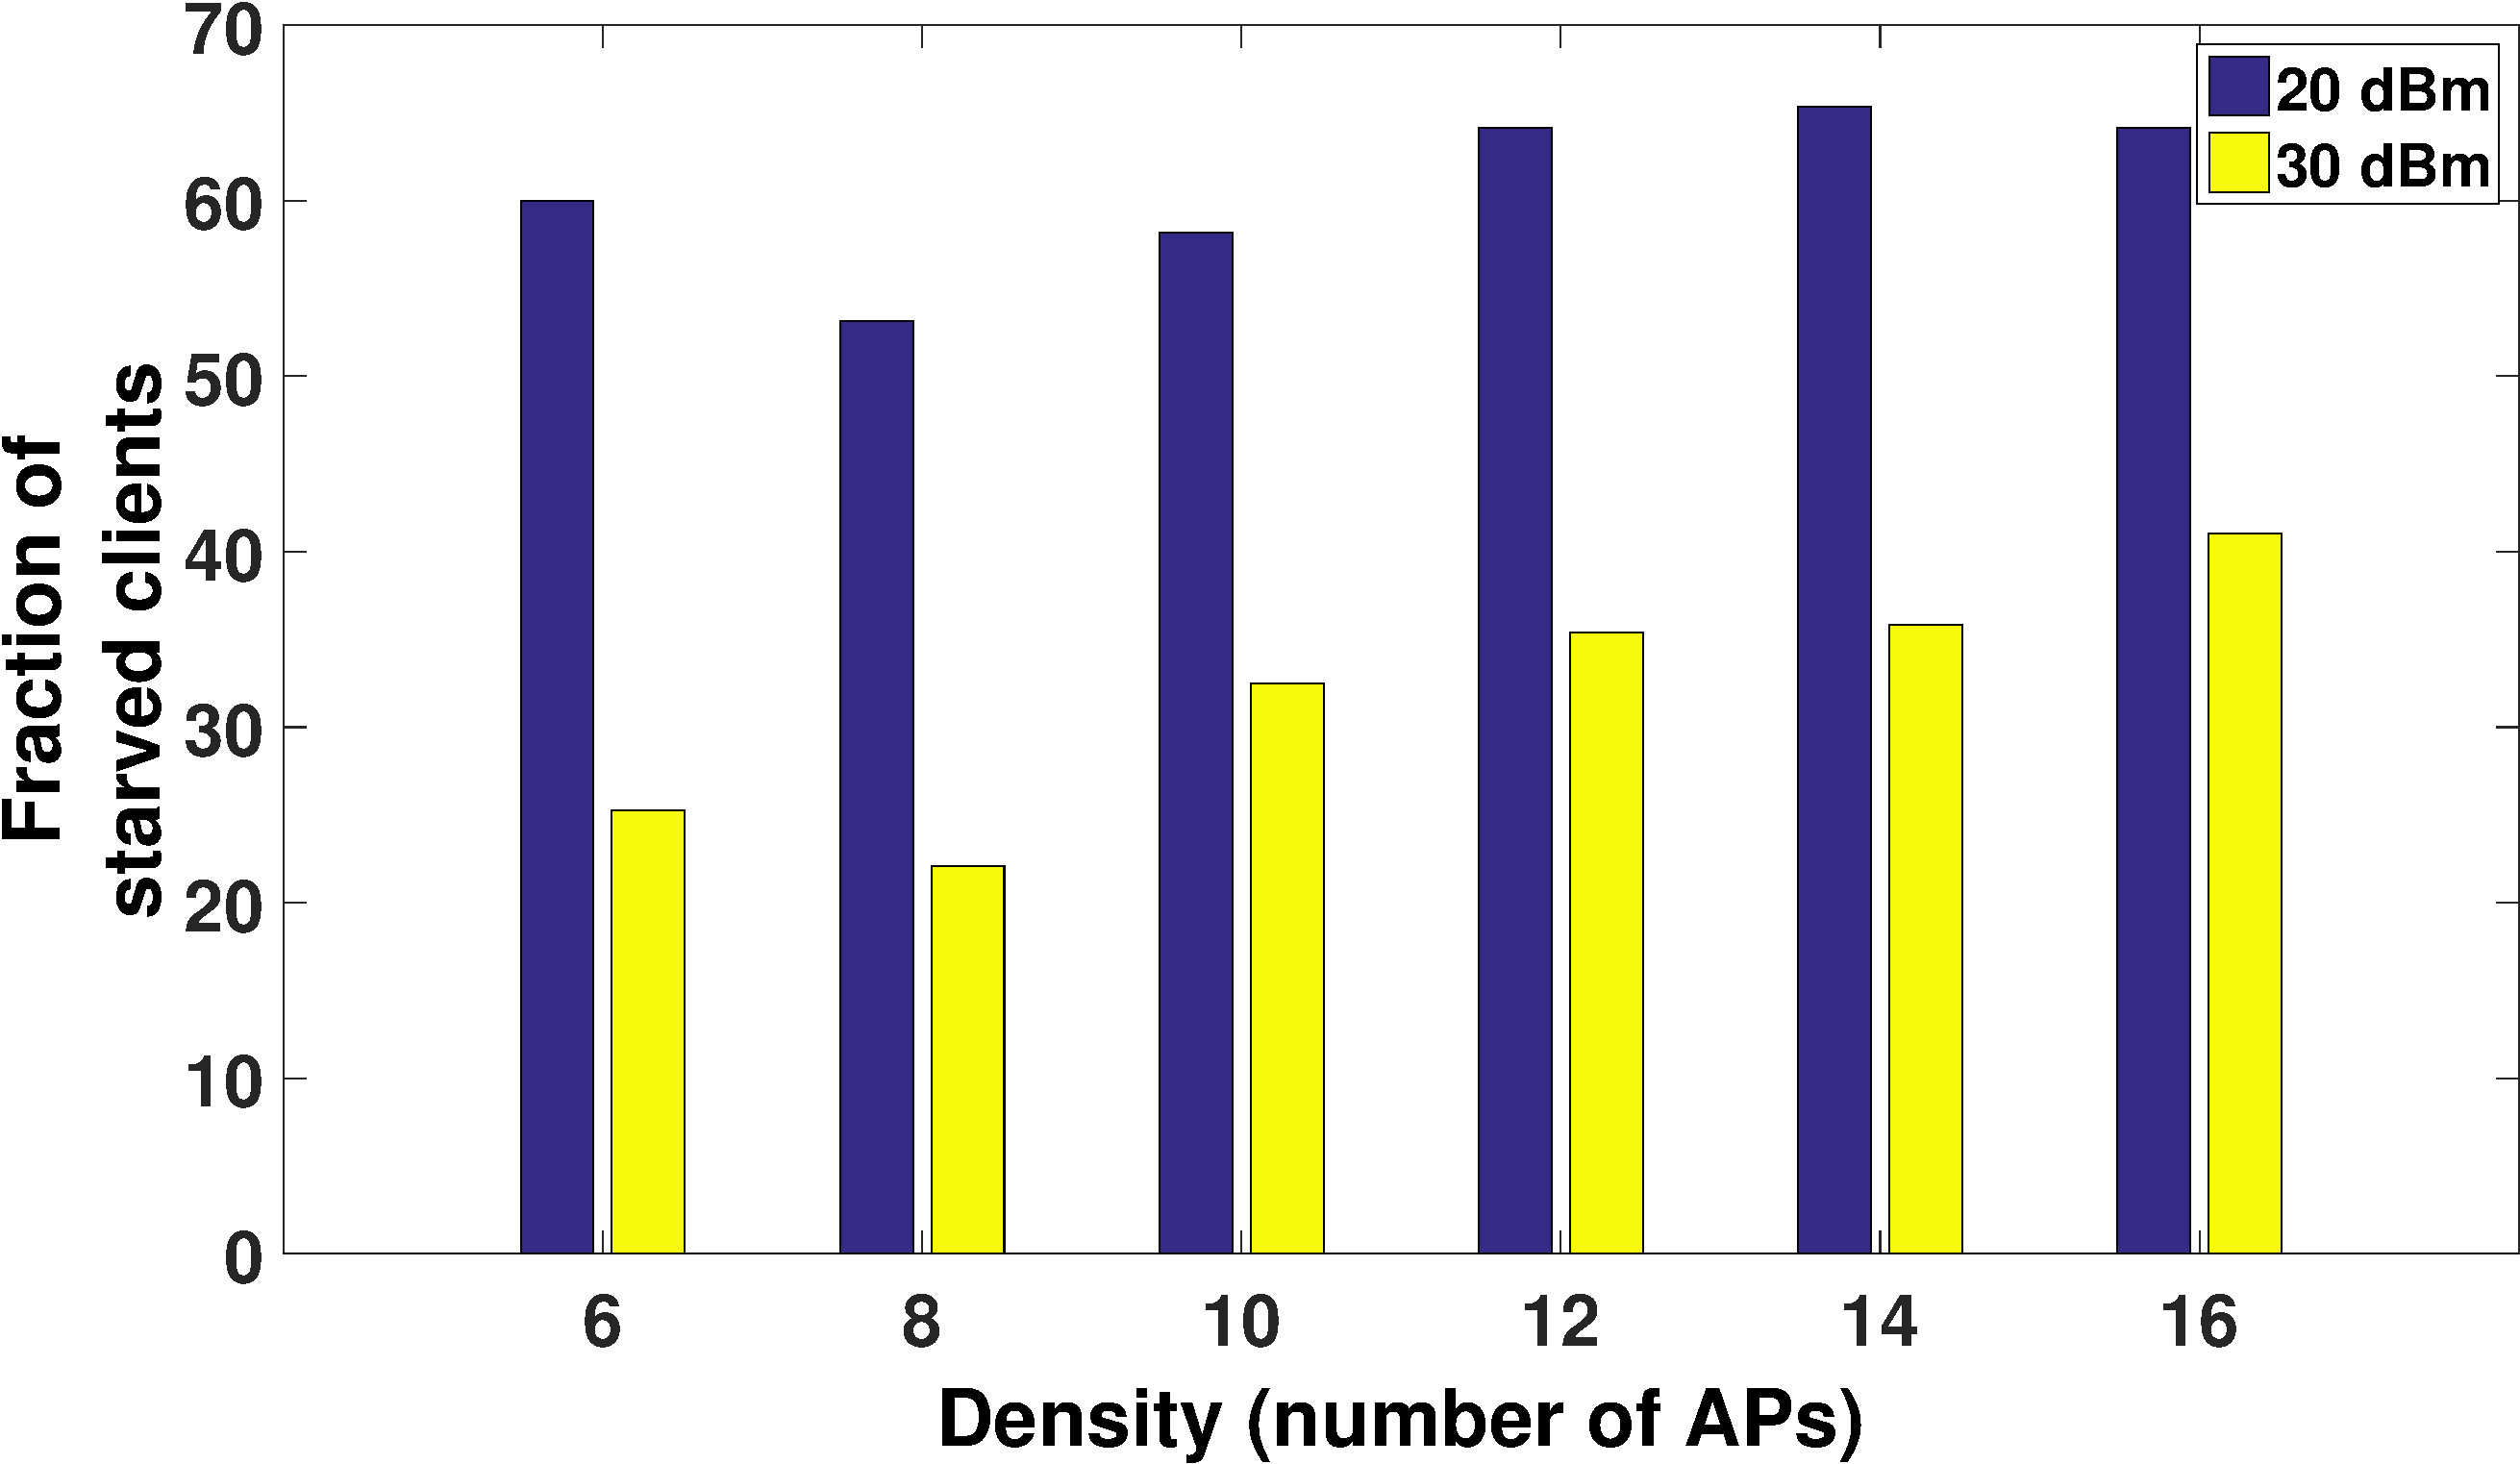
\includegraphics[width=\columnwidth, height=0.4\columnwidth]{./figs/WiFiComparison-crop}
%%     \vspace{-0.3in}
%%   \caption{Fraction of starved clients in a 802.11af deployment for different client transmit powers.}
%%   \label{fig:starved}
%% %\vspace{-36pt}
%% \end{figure}

\begin{figure}[t]
  \centering
    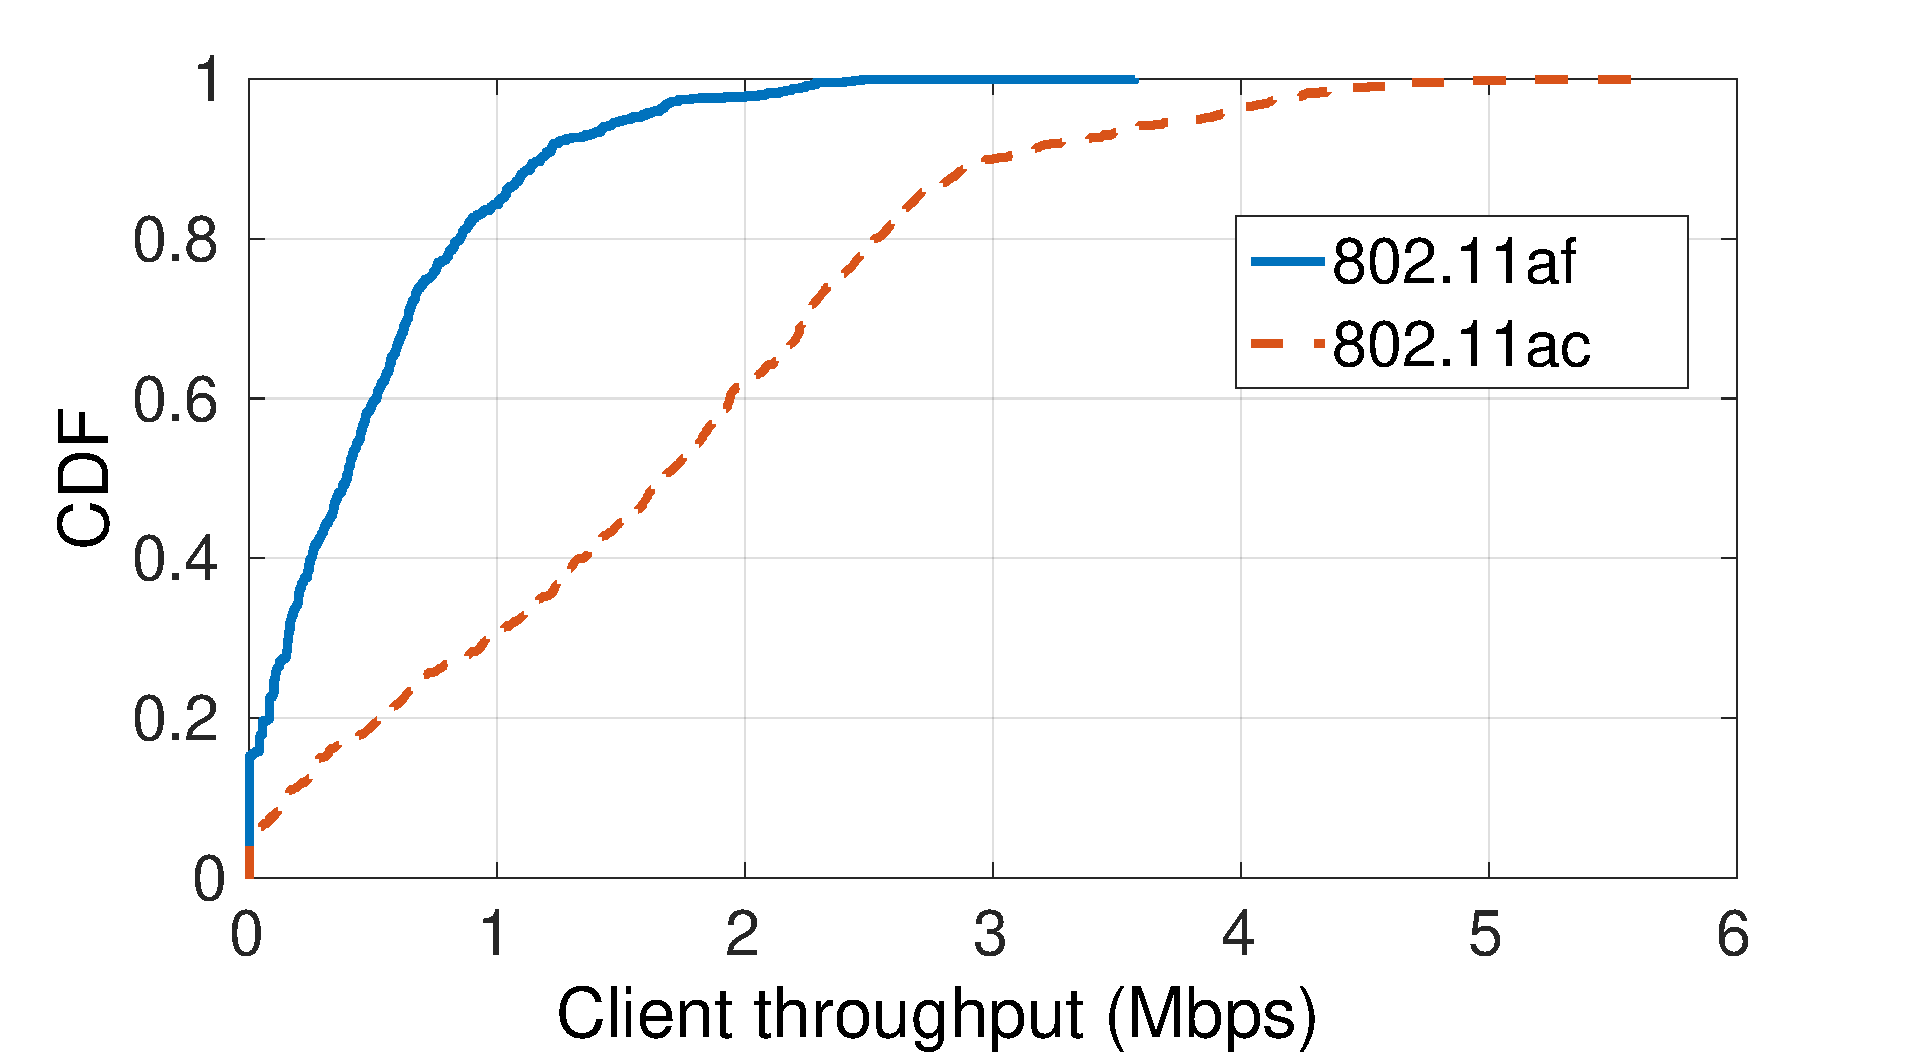
\includegraphics[width=\columnwidth, height=0.4\columnwidth]{./figs/af_vs_ac.pdf}
    \vspace{-0.3in}
  \caption{Wi-Fi MAC inefficiencies.}
  \label{fig:inefficiencies}
\vskip -8pt
\end{figure}



The 802.11af~\cite{Rice_af} standard inherits CSMA medium access mechanism from Wi-Fi, making it suitable for unplanned deployment. 
CSMA is able to use a channel whenever it is available, and quickly back off and adapt once other users are present. 

However, a number of well-known issues in \wf design render its deployment in TVWS problematic, such as hidden and exposed terminals and scheduling efficiency and fairness~\cite{idle_sense}.
These issues are even more pronounced in a long-range network. To illustrate this, we simulate 802.11af and 802.11ac networks in ns3 (please see Section~\ref{sec:eval} for details of simulation settings). 
In both cases we use 20 MHz channels, and we use RTS/CTS as we have observed that it improves performance. 
In both cases we consider the same network of access points and place the same number of clients within the corresponding range of each access point. 
The network range is smaller in case of 802.11ac (home Wi-Fi) than 802.11af (outdoor cellular) because of lower power (20dBm vs 36dBm) and worse propagation, 
but the average SNR at the receiver is same in both scenarios. 
However, the throughput of the 802.11af networks is much worse, as can be seen in Figure~\ref{fig:inefficiencies}.
Therefore, although CSMA offers efficient and fair contention resolution in shot-range Wi-Fi networks, this is far from obvious in the cellular scenario. \\

{\bf Summary.} Overall, LTE appears as a better fit for a TV white space cellular network due to its unique PHY and MAC layer properties.
However, it has never been fully considered as a candidate design due to its lack of uncoordinated interference management. We explore this by describing \cf over the next sections.




%% As already discussed, the links in TVWS networks are asymmetric, with APs transmitting at 30dBm power and mobiles
%% transmitting at 20dBm power, which significantly degrades carrier sensing. 
%% This is shown in Figure~\ref{fig:starved}, which shows
%% the fraction of starved clients for \wf in TVWS. The details of this experiment
%% can be found in Section~\ref{sec:eval}. 
%% The figure also reminds us that exposed and hidden terminal
%% inefficiencies are still present even when clients and APs use the
%% same transmit power (30 dBm in this example).




%% {\bf Ghufran, Lili: Write more about what are the reasons for poor WiFi's behaviour.}
%% \begin{figure}[t]
%%   \centering
%%     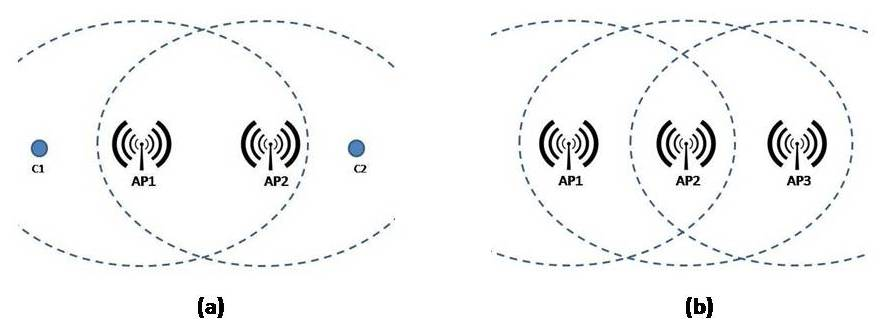
\includegraphics[width=\columnwidth, height=0.4\columnwidth]{./figs/wifi_inefficiencies.jpg}
%%     \vspace{-0.3in}
%%   \caption{CSMA inefficiencies.}
%%   \label{fig:inefficiencies}
%% %\vspace{-36pt}
%% \end{figure}
%% \begin{itemize}
%% \item {\bf Issues in uplink vs. downlink}\\
%% Figure~\ref{fig:inefficiencies} (a) shows an example in which AP1 is prevented from sending packets to its client (C1) because neighboring AP2 is transmitting to its client (C2). Ideally both APs should be able to send simultaneous downlink transmissions but Wi-Fi CSMA causes AP1 to conclude that it will interfere with the transmission by its neighbor AP2, However C1 can still receive the transmission of AP1 without interference because it is out of range of AP2. The primary reason for this issue is that for a downlink transmission the CSMA is done on the uplink instead. The simulation results for the scenario depicted in the figure show that this issue causes the total network throughput to be effectively halved of what it ideally should be.\\
%% \item { \bf Issues in multiple downlinks}\\
%% Wi-Fi guarantees an equal long term channel access probability to all hosts. This causes the throughput of all clients with higher bitrate to be reduced to the throughput of the client with lowest bit rate because The slower client gets a higher air time compared to the faster client, resulting in unfair resource allocation and overall throughput degradation of the network.
%% \item {\bf Issues in multiple APs}\\
%% Figure~\ref{fig:inefficiencies} (b) shows an example in which AP2 interferes with both AP1 and AP3, but AP1 and AP3 can not listen to each other's transmissions. In this scenario Wi-Fi CSMA would cause AP2 to starve if AP1 and AP2 do not transmit in a perfectly synchronized manner. This is because both AP1 and AP3 can transmit simultaneously and unless their transmissions end at the same time AP2 would always find the channel busy. The simulations results for the scenario depicted in the Figure show that AP2 manages to get an airtime of only around 3\% whereas AP1 and AP3 keep transmitting for the rest of the time.\\ 
%% \end{itemize}





%% \subsection{Towards an ideal design}
%% \label{sec:ideal}

%% In summary, both Wi-Fi and LTE have its deficiencies when applied to unlicensed cellular scenario in TV white spaces. 
%% However, LTE seems a better candidate yet it is rarely considered as a candidate design for TV white spaces. 
%% Wi-Fi design is inadequate for both PHY and MAC. 
%% LTE's PHY is well suited for long range and high bandiwidth. 
%% We next argue that LTE MAC and network layers can be adapted, with software modifications, to meet the other requirements of TV white space networking, such as decentralized interference management and channel selection through the database.


